\documentclass[tikz, border=5pt]{standalone}

% Semantic GitHub colors for the light theme.
% The Poe task embeds the dark palette from theme-dark.css into each SVG.
\usepackage{tikz}
\usepackage{amsmath, amssymb}
\usetikzlibrary{arrows.meta, calc, positioning, decorations.pathreplacing}

% Text and surfaces.
\definecolor{ghtext}{HTML}{1F2328}
\definecolor{ghmuted}{HTML}{59636E}
\definecolor{ghborder}{HTML}{D1D9E0}
\definecolor{ghpanel}{HTML}{F6F8FA}

% Accent colors and their softer backgrounds.
\definecolor{ghblue}{HTML}{0969DA}
\definecolor{ghbluesoft}{HTML}{DDF4FF}
\definecolor{ghgreen}{HTML}{1A7F37}
\definecolor{ghgreensoft}{HTML}{DAFBE1}
\definecolor{ghpurple}{HTML}{8250DF}
\definecolor{ghpurplesoft}{HTML}{FBEFFF}
\definecolor{ghorange}{HTML}{9A6700}
\definecolor{ghorangesoft}{HTML}{FFF8C5}
\definecolor{ghred}{HTML}{CF222E}
\definecolor{ghredsoft}{HTML}{FFEBE9}

\tikzset{
    >={Stealth[length=2.1mm, width=1.2mm]},
    card/.style={
        fill=ghpanel,
        draw=ghborder,
        rounded corners=2.6mm,
        line width=0.6pt,
    },
    heading/.style={font=\sffamily\small\bfseries, text=ghtext},
    regular/.style={font=\sffamily\small, text=ghtext},
    note/.style={font=\sffamily\footnotesize, text=ghmuted},
    tinylabel/.style={font=\sffamily\scriptsize, text=ghmuted},
    mathlabel/.style={font=\sffamily\small, text=ghtext},
    bluearrow/.style={-Stealth, draw=ghblue, line width=1.5pt},
    purplearrow/.style={-Stealth, draw=ghpurple, line width=1.4pt},
    thin/.style={draw=ghborder, line width=0.7pt},
}


\begin{document}
    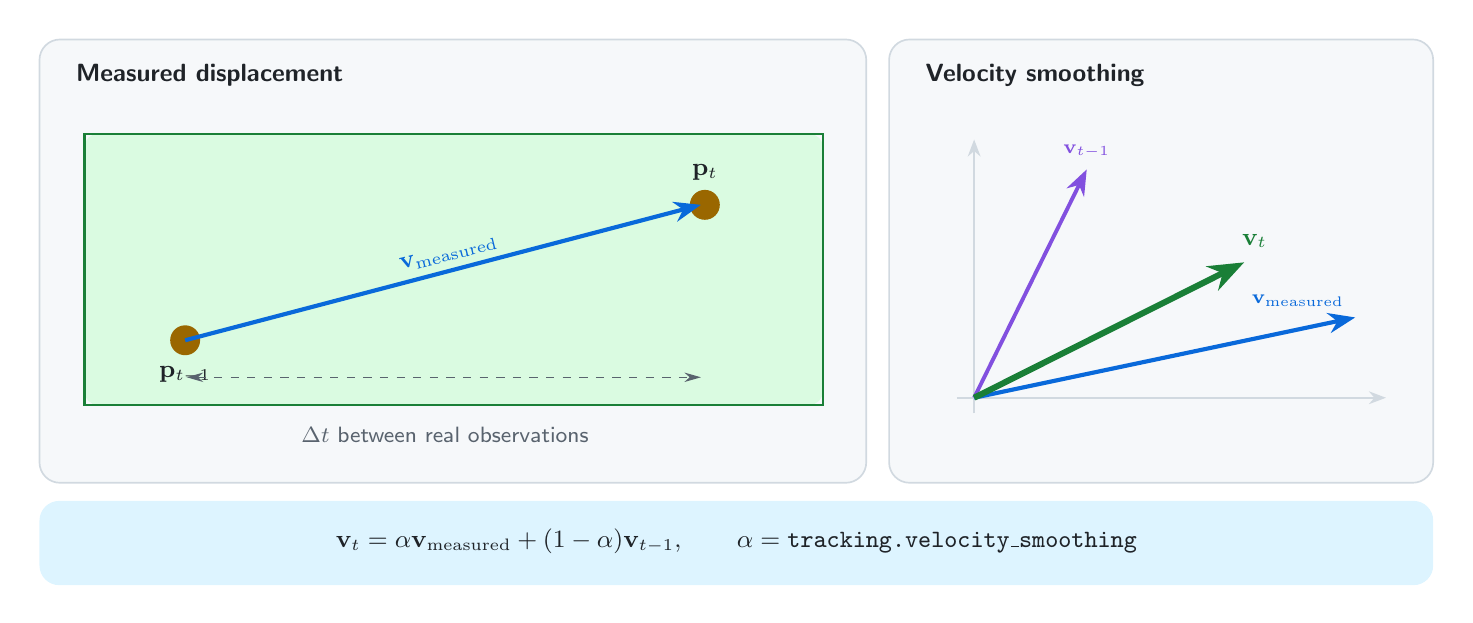
\begin{tikzpicture}[x=1cm, y=1cm]
        \path[use as bounding box] (0, 0) rectangle (18, 7.2);

        % Observations and velocity vectors.
        \draw[card] (0.15, 1.42) rectangle (10.65, 7.05);
        \draw[card] (10.94, 1.42) rectangle (17.85, 7.05);

        \node[heading, anchor=west] at (0.49, 6.6)
            {Measured displacement};
        \node[heading, anchor=west] at (11.28, 6.6)
            {Velocity smoothing};

        % Displacement between two real ball observations.
        \path[fill=ghgreensoft, rounded corners=1.7mm]
            (0.72, 2.41) rectangle (10.1, 5.85);
        \draw[ghgreen, line width=0.9pt]
            (0.72, 2.41) rectangle (10.1, 5.85);

        \fill[ghorange] (2, 3.23) circle (0.19);
        \fill[ghorange] (8.6, 4.95) circle (0.19);
        \node[mathlabel, anchor=north] at (2, 3.02) {$\mathbf p_{t-1}$};
        \node[mathlabel, anchor=south] at (8.6, 5.14) {$\mathbf p_t$};

        \draw[bluearrow] (2, 3.23) -- (8.55, 4.95);
        \node[mathlabel, text=ghblue, above, rotate=14]
            at (5.4, 4.12) {$\mathbf v_{\mathrm{measured}}$};
        \draw[ghmuted, <->, dashed]
            (2.02, 2.76) -- (8.55, 2.76);
        \node[note] at (5.3, 2.03)
            {$\Delta t$ between real observations};

        % Exponential smoothing: current, measured, and previous velocity.
        \coordinate (origin) at (12.02, 2.5);
        \draw[thin, -Stealth] (11.8, 2.5) -- (17.25, 2.5);
        \draw[thin, -Stealth] (12.02, 2.3) -- (12.02, 5.78);

        \draw[purplearrow] (origin) -- (13.45, 5.4)
            node[above, anchor=south, text=ghpurple,
                 font=\sffamily\scriptsize]
            {$\mathbf v_{t-1}$};
        \draw[bluearrow] (origin) -- (16.86, 3.52)
            node[above, anchor=south east, text=ghblue,
                 font=\sffamily\scriptsize]
            {$\mathbf v_{\mathrm{measured}}$};
        \draw[ghgreen, -Stealth, line width=2.2pt]
            (origin) -- (15.45, 4.22);
        \node[mathlabel, anchor=south west, text=ghgreen]
            at (15.3, 4.28) {$\mathbf v_t$};

        % Smoothing factor provided by the project configuration.
        \path[fill=ghbluesoft, rounded corners=2.5mm]
            (0.15, 0.12) rectangle (17.85, 1.19);
        \node[mathlabel] at (9, 0.68)
            {$\displaystyle\mathbf v_t=\alpha\mathbf v_{\mathrm{measured}}+(1-\alpha)\mathbf v_{t-1},\qquad\alpha=\texttt{tracking.velocity\_smoothing}$};
    \end{tikzpicture}
\end{document}
